\documentclass{article}

% WORKING DRAFT for section-by-section editing.
% Use `paper_template.tex` as the reusable blank structure.
% Main-track anonymous submission.
% Use `preprint` to show authors while drafting; remove for anonymous submission.
\usepackage[preprint]{neurips_2026}

\usepackage[utf8]{inputenc}
\usepackage[T1]{fontenc}
\usepackage{hyperref}
\usepackage{url}
\usepackage{booktabs}
\usepackage{amsfonts}
\usepackage{amsmath}
\usepackage{amssymb}
\usepackage{nicefrac}
\usepackage{microtype}
\usepackage{xcolor}
\usepackage{tikz}
\usetikzlibrary{positioning,arrows.meta}
\raggedbottom

\title{Knockout Evaluation of Hidden-Mechanic Discovery Under Partial Observability}

\author{%
  \begin{minipage}[t]{0.32\linewidth}\centering
    \textbf{Kaaustaaub Shankar} \\
    Independent
  \end{minipage}%
  \begin{minipage}[t]{0.32\linewidth}\centering
    \textbf{Edward Lue Chee Lip} \\
    Independent
  \end{minipage}%
  \begin{minipage}[t]{0.32\linewidth}\centering
    \textbf{Joshua Liu} \\
    Independent
  \end{minipage} \\[1.4em]
  \begin{minipage}[t]{0.32\linewidth}\centering
    \textbf{Ben Smith} \\
    Algoverse
  \end{minipage}%
  \begin{minipage}[t]{0.32\linewidth}\centering
    \textbf{Sean Wu} \\
    Algoverse
  \end{minipage}%
  \begin{minipage}[t]{0.32\linewidth}\centering
    \textbf{Kevin Zhu} \\
    Algoverse
  \end{minipage}
}

% HANDOFF NOTES: keep these centralized so later edits do not drift or break inline comments.
% - Related Work / references cover POMDP, ARC-AGI-3, and process-evaluation context;
%   keep `references.bib` synced if framing shifts.
% - All ka59simple cells are reported with Wilson 95% CIs; per-cell numbers come from
%   `scripts/wilson_cis.py` against `jkj results - Detailed_Results(1).csv`.
% - The pre-fix GPT-5.2 default-reasoning column (the "5.2 dflt" data, contaminated by an
%   OpenRouter reasoning_effort handler bug) is excluded from the main body and reported
%   only in Appendix~E for completeness.

\begin{document}

\maketitle

\begin{abstract}
Outcome metrics conflate task completion with discovery of latent task structure. We introduce a four-axis knockout framework---World, Goal, Mechanics, Feedback---that ablates the agent's observation, goal specification, transition dynamics, and per-turn feedback signal one axis at a time. We instantiate the framework on the KA59 family of ARC-AGI environments: canonical KA59 yields $0\%$ wins for every tested model and reasoning setting, so we introduce \texttt{ka59simple}, a single-goal variant that preserves KA59's hidden \emph{wall-transfer} mechanic (an engine asymmetry that lets pushed objects pass through walls), as our primary attributed comparison.

Across GPT-5.2 and Grok-4.1-fast under three reasoning settings, three findings hold. First, world- and mechanics-axis ablations consistently collapse win rate to $0\%$ ($95\%$ upper bounds $\le 43\%$ at $n=5$), partly entailed by the binary-knockout design; a uniform-random agent achieves $0/50$ wins on \texttt{ka59simple}, calibrating model performance well above floor. Second, the goal axis shows the largest cross-family reasoning interaction at the point-estimate level: at $n=10$, GPT-5.2 drops $60\% \to 20\%$ from no-reasoning to medium while Grok rises $20\% \to 70\%$ on the same cell---a $90$pp directional swing, although within-family $95\%$ confidence intervals overlap. Third, verbal and behavioral signatures of mechanic discovery decouple completely: across $210$ \texttt{ka59simple} trials, $56$ wins required exploiting the wall-transfer mechanic, but a heuristic verbal-discovery regex (not human-validated) never fired, and a procedural OODA-F scaffold (an explicit observe/orient/decide/act loop with forced-reframe directives) yields $0/16$ wins despite eliciting regular hypothesis revision.

BP35 and LS20 supporting evidence (GPT-5.2 only) is consistent with the world-axis collapse pattern. Together, these results indicate that hidden-mechanic discovery is a distinct capability axis on which self-report-based metrics systematically underestimate behavioral exploitation.
\end{abstract}

\section{Introduction}
Recent agent evaluations frequently report whether a model eventually solves a task, reaches a goal, or achieves a high final score. In interactive environments with hidden rules, however, terminal outcome alone is an incomplete measure of competence. Two agents can reach the same outcome for very different reasons: one by inferring the latent transition structure of the environment, another by stumbling onto a successful behavior without ever forming a corresponding internal model. Conversely, an agent may form a partially correct hypothesis and still fail under finite turn budgets. If the scientific question concerns interactive reasoning under partial observability, the evaluation must distinguish task completion from latent-mechanic discovery.

We approach this problem by adapting a partially observable Markov decision process (POMDP) lens to benchmark design. Many components of a real-world agent task are not directly given to the agent: parts of the world state may be hidden, the reward (objective) may be implicit, the transition function (mechanics) may be opaque, and the per-step feedback signal may be impoverished. We organize these four directions of underspecification into a knockout framework with four axes: \emph{World}, \emph{Goal}, \emph{Mechanics}, and \emph{Feedback}. A baseline condition presents all four in their most informative form; each single-axis knockout removes one in its entirety while leaving the others fixed. The framework lets us ask not only whether an agent succeeds, but which missing source of specification disrupts discovery.

To pair outcome metrics with discovery-sensitive signals, we report four classes of measurements: terminal win rate, an environment-specific partial-progress metric (max simultaneous goals occupied), a behavioral discovery indicator (the count of \emph{wall-transfer events}---a signature of the hidden KA59 mechanic), and a verbal-discovery indicator computed from a regular-expression scan over the agent's stated hypotheses (where the agent emits them). The behavioral and verbal indicators are designed to be commensurable on the same trials.

Empirically, this paper focuses on the KA59 lane of an ARC-AGI-style benchmark family. Canonical KA59 yields $0\%$ wins for every tested model and reasoning setting and serves as a difficulty anchor. For attributed axis comparisons, we introduce \texttt{ka59simple}, a single-goal variant that removes the second goal tile while preserving the hidden wall-transfer mechanic and the core pusher--pushee interaction. We treat \texttt{ka59simple} as a methodological tool, not a benchmark replacement. BP35 and LS20 remain in scope as supporting environments rather than co-equal quantitative pillars.

Our contributions are:
\begin{itemize}
  \item A four-axis POMDP-grounded knockout framework that maps each axis to a component of the POMDP tuple, operationalized as binary ablations rather than graded reductions (Section~\ref{sec:pomdp}, Section~\ref{sec:method}).
  \item An attributed empirical study on \texttt{ka59simple} across two model families and three reasoning settings, with Wilson 95\% confidence intervals on every cell, a uniform-random floor reference ($0/50$ wins), and a partial-progress metric (Section~\ref{sec:experiments}).
  \item A trace-level analysis showing complete verbal/behavioral decoupling of mechanic discovery in our dataset---behavioral exploitation occurs without verbal discovery, and a procedural OODA-F scaffold does not close the gap (Section~\ref{sec:verbal-behavioral}).
  \item An explicit knockout-severity disclosure (Appendix~\ref{app:severity}) and full prompts (Appendix~\ref{app:prompts}), so that the binary-knockout design and its limits are reproducible.
\end{itemize}

\section{Related Work}
\label{sec:related}
This work sits at the intersection of planning under partial observability, interactive ARC-style benchmarks, agentic benchmark design, exploration under hidden structure, and process-level trajectory analysis.

Classic POMDP theory formalizes decision making when state is only partially observed \citep{kaelbling1998pomdp}. Recent practitioner-oriented work argues that many LLM applications are best understood as POMDP-like systems whose surrounding scaffolding must track history, latent state, and feedback rather than as monolithic ``agents'' \citep{tensorzero2025pomdp}. Our four-axis knockout framing operationalizes that intuition into a diagnostic evaluation: each axis isolates a different component of the underlying POMDP tuple.

The Abstraction and Reasoning Corpus (ARC) was introduced to probe generalization via abstraction and core-knowledge priors \citep{chollet2019measure}. ARCLE recast ARC as an interactive learning environment for reinforcement learning agents \citep{lee2025arcle}. ARC-AGI-3 pushes this trajectory further by defining instruction-free, turn-based environments in which agents must explore, infer goals, build internal models of dynamics, and plan under sparse feedback \citep{arcfoundation2026arcagi3}. Our setting is closest to this interactive ARC line, but our focus is diagnostic rather than leaderboard-oriented: we ask which part of the task specification is missing and whether the agent discovers the latent mechanic required for success. Recent ARC-AGI-3 analyses likewise emphasize the importance of systematic exploration and world-model formation \citep{arcprize2026analysis,rudakov2025grapharc}.

A parallel line evaluates language agents in interactive environments---WebShop, AgentBench, SmartPlay, BALROG, AgentQuest, and TheAgentCompany study grounded web interaction, games, and broader workflows \citep{yao2022webshop,liu2024agentbench,wu2023smartplay,paglieri2024balrog,gioacchini2024agentquest,xu2024agentcompany}. These benchmarks expose failures invisible in static QA but typically report aggregate task success rather than isolating whether collapse comes from observability, objective specification, latent dynamics, or feedback. Our knockout design directly targets that gap.

Exploration under sparse, delayed, or deceptive feedback has been studied through curiosity-driven methods, Go-Explore, and world-model approaches \citep{pathak2017curiosity,ecoffet2019goexplore,ha2018worldmodels}. We borrow the motivation but use it to structure a benchmark methodology rather than to propose an exploration algorithm.

Our use of behavioral and verbal discovery indicators is closest to process- and trajectory-level evaluation. ReAct showed that interleaving reasoning traces with actions can produce more interpretable interactive trajectories \citep{yao2023react}; process-supervision and process-evaluation work argues for assessing intermediate reasoning and behavior rather than only final answers \citep{lightman2024verify,kuang2025enconda,gritta2026processeval}. Our indicators are lighter-weight and behavior-grounded: a count of mechanic-triggering events on the environment side, paired with a regex over the agent's stated hypotheses on the verbal side. We do not claim our regex is a faithful estimator of model belief; we use it precisely to expose its disagreement with behavior.

\section{POMDP Formalism and Knockout Mapping}
\label{sec:pomdp}
We model an environment instance as a partially observable Markov decision process $\mathcal{M} = \langle \mathcal{S}, \mathcal{A}, \mathcal{O}, T, Z, R, \gamma \rangle$, where $\mathcal{S}$ is the ground-truth state space (positions of all sprites, level index, step budget), $\mathcal{A}$ is the agent's action space (\texttt{MOVE\_\{UP,DOWN,LEFT,RIGHT\}} and \texttt{CLICK} with a target position), $T : \mathcal{S} \times \mathcal{A} \to \Delta\mathcal{S}$ is the environment transition kernel (which encodes the latent wall-transfer asymmetry described in Section~\ref{sec:ka59}), $\mathcal{O}$ is the observation space presented to the agent each turn, $Z : \mathcal{S} \to \Delta\mathcal{O}$ is the observation function constructed by the harness, $R$ is a sparse reward (level win or game-over), and $\gamma$ is implicit in the finite turn budget.

The four knockout axes correspond to deliberate ablations of these components, communicated entirely through the system prompt and the per-turn observation:
\begin{itemize}
  \item \textbf{World} $\leftrightarrow Z$: in \texttt{WORLD\_HARD}, the observation function is restricted---non-player object positions are removed, leaving only the selected piece's position, four directional ``blocked'' flags, level/budget counters, and total counts of objects per category.
  \item \textbf{Goal} $\leftrightarrow R$: in \texttt{GOAL\_HARD}, the system prompt provides no description of the reward---the agent receives no statement of what counts as winning.
  \item \textbf{Mechanics} $\leftrightarrow T$: in \texttt{MECHANICS\_HARD}, the system prompt provides no description of $T$---no mention of pushing, walls, multi-selectables, coordinate system, or the \texttt{CLICK} action's semantics. The action protocol survives only as a one-line response-format instruction (Appendix~\ref{app:severity}).
  \item \textbf{Feedback}: in \texttt{FEEDBACK\_HARD}, the per-turn outcome description is replaced with the literal string \texttt{"Ok."}---the agent must infer outcomes from observation deltas alone.
\end{itemize}
A baseline condition presents all four axes in their most informative form (\texttt{EASY}). Each single-axis knockout sets exactly one axis to \texttt{HARD} while the other three remain at \texttt{EASY}. The underlying $\mathcal{M}$ does not change between conditions; only what the agent is told changes. Combined knockouts are possible but are not the focus of this paper. Figure~\ref{fig:axis-map} summarizes the mapping from POMDP components to axes to the corresponding prompt or observation ablation.

\begin{figure}[t]
  \centering
  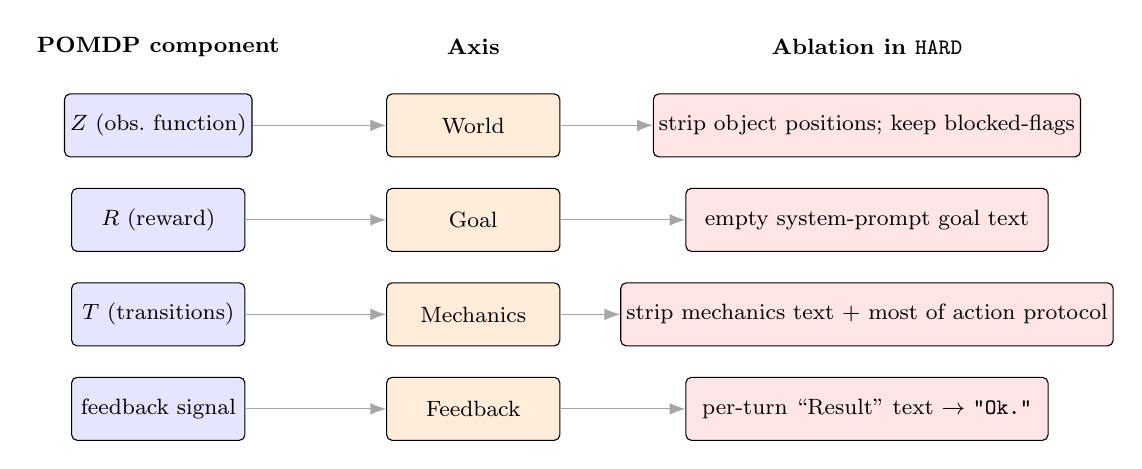
\begin{tikzpicture}[
    node distance=4mm and 8mm,
    box/.style={draw, rounded corners=2pt, minimum width=22mm, minimum height=8mm,
                font=\footnotesize, align=center, inner sep=2pt},
    pomdp/.style={box, fill=blue!10},
    axis/.style ={box, fill=orange!15},
    abl/.style  ={box, fill=red!10, minimum width=46mm},
    arr/.style  ={-{Latex[length=2mm]}, gray!70}
  ]
    % column headers
    \node[font=\footnotesize\bfseries] (h1) at (0, 4.5) {POMDP component};
    \node[font=\footnotesize\bfseries] (h2) at (4, 4.5) {Axis};
    \node[font=\footnotesize\bfseries] (h3) at (9, 4.5) {Ablation in \texttt{HARD}};

    % pomdp components
    \node[pomdp] (Z) at (0, 3.5) {$Z$ (obs.\ function)};
    \node[pomdp] (R) at (0, 2.3) {$R$ (reward)};
    \node[pomdp] (T) at (0, 1.1) {$T$ (transitions)};
    \node[pomdp] (F) at (0,-0.1) {feedback signal};

    % axes
    \node[axis] (W) at (4, 3.5) {World};
    \node[axis] (G) at (4, 2.3) {Goal};
    \node[axis] (M) at (4, 1.1) {Mechanics};
    \node[axis] (Fa) at (4,-0.1) {Feedback};

    % ablations
    \node[abl] (aW) at (9, 3.5) {strip object positions; keep blocked-flags};
    \node[abl] (aG) at (9, 2.3) {empty system-prompt goal text};
    \node[abl] (aT) at (9, 1.1) {strip mechanics text + most of action protocol};
    \node[abl] (aF) at (9,-0.1) {per-turn ``Result'' text $\to$ \texttt{"Ok."}};

    \foreach \a/\b in {Z/W, R/G, T/M, F/Fa} \draw[arr] (\a) -- (\b);
    \foreach \a/\b in {W/aW, G/aG, M/aT, Fa/aF} \draw[arr] (\a) -- (\b);
  \end{tikzpicture}
  \caption{The four-axis knockout framework operationalizes a POMDP-component-level ablation. Each axis targets a distinct component of the underlying $\mathcal{M} = \langle \mathcal{S}, \mathcal{A}, \mathcal{O}, T, Z, R, \gamma \rangle$ by removing or replacing the corresponding prompt or observation field. The action space $\mathcal{A}$ and the latent state $\mathcal{S}$ are not directly ablated; the table at right summarizes what changes in each \texttt{HARD} condition. See Appendix~\ref{app:severity} for the exact deltas.}
  \label{fig:axis-map}
\end{figure}

We deliberately operationalize each axis as a binary ablation rather than a graded reduction. This makes the design and its semantics explicit: ``\texttt{world\_hard} collapses performance'' is then a finding about how badly performance suffers when $Z$ is severely restricted, not about a continuous severity gradient. Appendix~\ref{app:severity} reproduces the exact prompt deltas and discusses confounds, particularly that \texttt{MECHANICS\_HARD} also removes the description of the \texttt{CLICK} target-position protocol. Findings on the mechanics axis should be interpreted with this confound in mind.

\section{The KA59 Family}
\label{sec:ka59}
KA59 is a turn-based ARC-AGI environment built on a sokoban-like physics engine. The agent controls one of one or more \emph{selectable} pieces and chooses among five action types: four directional moves (\texttt{MOVE\_\{UP,DOWN,LEFT,RIGHT\}}) and a \texttt{CLICK} action that takes a target position in pixel/grid coordinates. A level is won when every \emph{goal} tile on the board is simultaneously occupied by a selectable piece. Walls block movement; pushable objects (other selectables and blocks) shift one cell ahead of the player when the player tries to move into them.

\paragraph{Hidden mechanic.}
Canonical KA59 contains a deliberate engine asymmetry, illustrated in Figure~\ref{fig:wall-transfer}: the move handler used by the player checks for wall tags and silently reverts blocked moves, but the recursive push handler used to propagate motion through pushed sprites \emph{does not check walls}. Consequently, when the player pushes a second selectable into a wall, the pushed sprite passes through to the cell on the far side. We refer to this as the \emph{wall-transfer mechanic}. Producing it requires a multi-step plan: arrange one selectable on each side of a wall, push the pushable one through, switch control to the transferred sprite via \texttt{CLICK}, and then complete navigation. None of the prompts (including \texttt{MECHANICS\_EASY}) describe this asymmetry; instead, \texttt{MECHANICS\_EASY} states only that ``not all wall-like boundaries behave identically---you must interact with them to discover their behavior.'' The asymmetry is the discovery signal the benchmark is designed to elicit.

\begin{figure}[t]
  \centering
  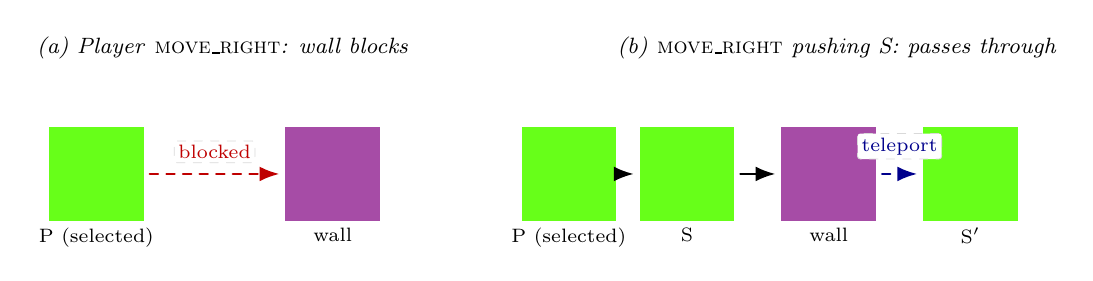
\begin{tikzpicture}[
    cell/.style    ={draw=none, minimum size=12mm, inner sep=0pt},
    sel/.style     ={cell, fill=green!55!lime!90},     % selectable, matches game
    wall/.style    ={cell, fill=violet!70, text=white}, % wall
    arr/.style     ={-{Latex[length=2.5mm]}, thick, line cap=round},
    block/.style   ={arr, red!75!black, dashed},
    pass/.style    ={arr, blue!55!black, dashed},
    title/.style   ={font=\footnotesize\itshape, align=center},
    arrlab/.style  ={font=\scriptsize, inner sep=1.5pt, fill=white,
                     rounded corners=1pt, draw=black!15, line width=0.3pt},
    celllab/.style ={font=\scriptsize, anchor=north, inner sep=2pt}
  ]
    % --- Panel A: MOVE blocked ---
    \node[title] at (2.2, 3.0) {(a) Player \textsc{move\_right}: wall blocks};
    \node[sel]  (pa) at (0.6, 1.4) {};
    \node[wall] (wa) at (3.6, 1.4) {};
    \node[celllab] at (pa.south) {P (selected)};
    \node[celllab] at (wa.south) {wall};
    \draw[block] ([xshift=2pt]pa.east) -- ([xshift=-2pt]wa.west)
      node[arrlab, midway, yshift=8pt]{blocked};

    % --- Panel B: PUSH passes through ---
    \node[title] at (10.0, 3.0) {(b) \textsc{move\_right} pushing S: passes through};
    \node[sel] (pb)  at (6.6, 1.4)  {};
    \node[sel] (sb)  at (8.1, 1.4)  {};
    \node[wall] (wb) at (9.9, 1.4)  {};
    \node[sel] (sb2) at (11.7, 1.4) {};
    \node[celllab] at (pb.south)  {P (selected)};
    \node[celllab] at (sb.south)  {S};
    \node[celllab] at (wb.south)  {wall};
    \node[celllab] at (sb2.south) {S$'$};
    \draw[arr] ([xshift=2pt]pb.east)  -- ([xshift=-2pt]sb.west);
    \draw[arr] ([xshift=2pt]sb.east)  -- ([xshift=-2pt]wb.west);
    \draw[pass] ([xshift=2pt]wb.east) -- ([xshift=-2pt]sb2.west)
      node[arrlab, midway, yshift=10pt]{teleport};
  \end{tikzpicture}
  \caption{The wall-transfer asymmetry in the KA59 engine. Green tiles are selectable pieces (matching the game's visual); purple tiles are walls. P denotes the currently selected piece (the player); S denotes a non-selected selectable. (a) When the player (P) attempts to step onto a wall cell, the move handler checks the wall tag and reverts the action. (b) When the same \textsc{move\_right} would propagate through a pushed second selectable (S), the recursive push handler does not check wall tags, and S is teleported to the far side of the wall (S$'$). A win requires triggering case (b) and then transferring selection to S$'$ via \texttt{CLICK}.}
  \label{fig:wall-transfer}
\end{figure}

\paragraph{Canonical KA59 vs.~\texttt{ka59simple}.}
Canonical KA59 has seven levels and two goal tiles per relevant level. The shortest known win path is approximately twelve actions and requires the wall-transfer mechanic plus a CLICK-based perspective switch. We confirmed empirically that the canonical level is solvable in $\sim$$12$ actions; under our settings, however, it is not solved by any tested LLM ($0\%$ across $n=5$ in five conditions, two reasoning settings, two model families). To enable axis-attributed comparisons, we constructed \texttt{ka59simple} (Figure~\ref{fig:board}, Appendix~\ref{app:envs}) by removing the second (left) goal tile from level~1 while preserving both selectables, the wall, and the wall-transfer asymmetry. The optimal solve is six actions and still requires triggering the hidden mechanic. \texttt{ka59simple} is a methodological tool, not a benchmark replacement; canonical KA59 remains the authoritative anchor for the hardest-case effect.

\begin{figure}[t]
  \centering
  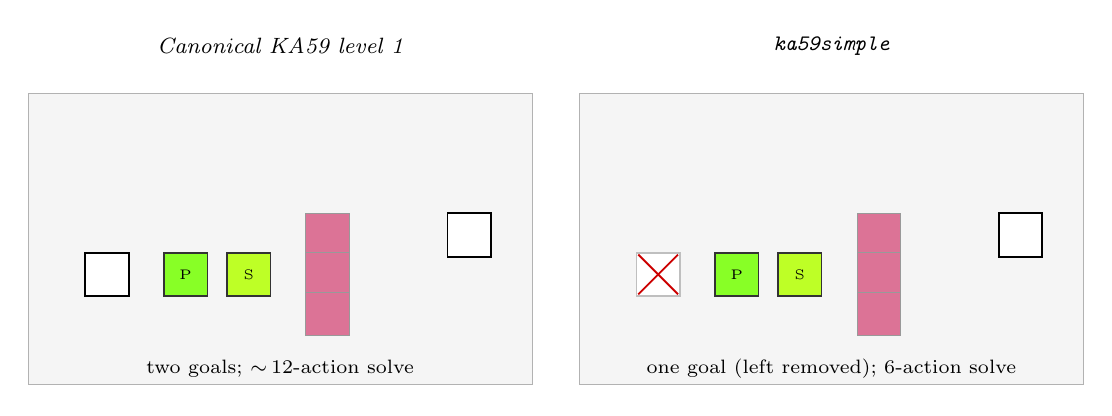
\begin{tikzpicture}[
    floor/.style={draw=black!40, line width=0.3pt, minimum size=5.5mm, fill=white,
                  inner sep=0pt, font=\tiny},
    walltile/.style ={floor, fill=purple!55},
    selA/.style     ={floor, fill=green!55!yellow!85, line width=0.6pt, draw=black!80},
    selB/.style     ={floor, fill=green!30!yellow!85, line width=0.6pt, draw=black!80},
    goalbox/.style  ={floor, draw=black, line width=0.7pt},
    title/.style    ={font=\footnotesize\itshape, align=center},
    pcap/.style     ={font=\scriptsize}
  ]
    % --- canonical KA59 panel ---
    \node[title] at (3.0, 4.1) {Canonical KA59 level 1};
    \begin{scope}[shift={(0,0)}]
      % background floor
      \draw[fill=black!4, draw=black!30] (-0.2,-0.2) rectangle (6.2, 3.5);
      % left goal at ~(2,23) → put at left
      \node[goalbox] (gL) at (0.8, 1.2) {};
      % left selectable at (9,21)
      \node[selA] (sLa) at (1.8, 1.2) {P};
      % right selectable at (18,21)
      \node[selB] (sLb) at (2.6, 1.2) {S};
      % wall (vertical bar) at (24,12)
      \node[walltile] (wL) at (3.6, 1.7) {};
      \node[walltile] at (3.6, 1.2) {};
      \node[walltile] at (3.6, 0.7) {};
      % right goal at (35,17)
      \node[goalbox] (gR) at (5.4, 1.7) {};
      % path label
      \node[pcap] at (3.0, 0.0) {two goals; $\sim$\,12-action solve};
    \end{scope}

    % --- ka59simple panel ---
    \node[title] at (10.0, 4.1) {\texttt{ka59simple}};
    \begin{scope}[shift={(7,0)}]
      \draw[fill=black!4, draw=black!30] (-0.2,-0.2) rectangle (6.2, 3.5);
      % left goal removed - draw it greyed out with a red X
      \node[goalbox, draw=black!25] (gLs) at (0.8, 1.2) {};
      \draw[red!80!black, line width=0.7pt]
        ([xshift=1pt,yshift=1pt]gLs.south west) -- ([xshift=-1pt,yshift=-1pt]gLs.north east);
      \draw[red!80!black, line width=0.7pt]
        ([xshift=-1pt,yshift=1pt]gLs.south east) -- ([xshift=1pt,yshift=-1pt]gLs.north west);
      % left selectable
      \node[selA] (sLa2) at (1.8, 1.2) {P};
      % right selectable
      \node[selB] (sLb2) at (2.6, 1.2) {S};
      % wall
      \node[walltile] at (3.6, 1.7) {};
      \node[walltile] at (3.6, 1.2) {};
      \node[walltile] at (3.6, 0.7) {};
      % right goal kept
      \node[goalbox] at (5.4, 1.7) {};
      \node[pcap] at (3.0, 0.0) {one goal (left removed); 6-action solve};
    \end{scope}
  \end{tikzpicture}
  \caption{Schematic of the canonical KA59 level~1 layout (left) versus our \texttt{ka59simple} variant (right). P and S denote the two selectable pieces; the purple bar is a wall block; black-outlined squares are goal tiles. \texttt{ka59simple} removes only the left goal (red cross), leaving the wall, both selectables, and the engine's hidden push-through-wall asymmetry intact. The optimal canonical solve is $\sim$$12$ actions and requires occupying both goals simultaneously; \texttt{ka59simple} reduces this to a $6$-action single-goal sequence that still requires triggering the wall-transfer mechanic. Distances and proportions are illustrative; exact pixel coordinates are listed in Appendix~\ref{app:envs}.}
  \label{fig:board}
\end{figure}

\paragraph{BP35 and LS20.}
BP35 and LS20 are two further ARC-AGI-style environments owned by other authors. They share the four-axis condition definitions and the action-protocol shape but differ in latent mechanics and goal structure. Their per-trial coverage is smaller and currently limited to GPT-5.2 and GPT-4.1; we use them as supporting evidence for the world-axis collapse pattern but not for cross-family or reasoning-effort claims.

\section{Knockout Methodology}
\label{sec:method}
\subsection{Conditions}
Each benchmark condition is a tuple $(\text{world}, \text{goal}, \text{mechanics}, \text{feedback}) \in \{\text{EASY}, \text{HARD}\}^4$ together with an environment $e \in \{\text{ka59}, \text{ka59simple}, \text{bp35}, \text{ls20}\}$ and a model configuration. Our primary conditions are baseline (all \texttt{EASY}) plus the four single-axis knockouts. We additionally report two procedural-mechanics variants on \texttt{ka59simple}: \texttt{mech\_ooda} and \texttt{mech\_ooda\_f} (Appendix~\ref{app:prompts}), discussed in Section~\ref{sec:reasoning}.

\subsection{Models and reasoning settings}
We compare GPT-5.2 (\texttt{openai/gpt-5.2}) and Grok-4.1-fast (\texttt{x-ai/grok-4.1-fast}), both routed through OpenRouter, under three reasoning configurations: explicit \texttt{none}, explicit \texttt{medium}, and an omitted-default (provider-side) setting. The omitted-default GPT-5.2 cells were collected before a per-handler bug in the OpenRouter reasoning-effort path was corrected, and so map to provider-default reasoning rather than to a controlled level. We report explicit \texttt{none} vs.\ \texttt{medium} as the primary within-family comparison and relegate the omitted-default cells to Appendix~\ref{app:cells}.

\subsection{Metrics}
We report four classes of measurement:
\begin{itemize}
  \item \textbf{Outcome}: win rate (with Wilson 95\% confidence intervals at the cell level) and average turns to win.
  \item \textbf{Partial progress}: average maximum goals simultaneously occupied within a trial (\texttt{max\_goals\_occupied}). On \texttt{ka59simple} this lies in $\{0, 1\}$ (single goal); on canonical KA59, in $\{0, 1, 2\}$.
  \item \textbf{Behavioral discovery}: total count of \emph{wall-transfer events}---turns on which the engine moved a non-player sprite by more than one cell, signalling that the wall-transfer asymmetry was triggered. We also track \texttt{object\_pushes} (within-cell pushes that respect walls).
  \item \textbf{Verbal discovery}: a regular-expression check over the agent's per-turn \texttt{orient} field (when emitted, i.e.\ in OODA and OODA-F conditions). Patterns target unambiguous push-through phrasing, with explicit veto patterns for \texttt{CLICK}-based misattribution. Full pattern list in Appendix~\ref{app:regex}.
\end{itemize}
We use \emph{behavioral discovery} and \emph{verbal discovery} in this paper rather than the more loaded term \emph{epistemic traces}; we revisit the relationship between the two in Section~\ref{sec:verbal-behavioral}.

\subsection{Trial structure}
Each trial runs a single instance of the chosen environment with a fixed turn budget. \texttt{ka59simple} uses a $32$-turn budget for one level; canonical KA59 uses a $50$-turn budget per level for one level (we restrict to level~1 throughout). The agent receives the system prompt once at start and an updated user prompt every turn (status, observation, recent action history). At the end of each run, the agent is asked to summarize its understanding of the goal and mechanics; this is logged but not used as a metric.

\section{Experiments}
\label{sec:experiments}
\subsection{Floor reference: uniform-random agent}
\label{sec:random}
To calibrate model performance, we ran a uniform-random policy on each environment whose source is in our repository. Each turn samples uniformly from \{\texttt{MOVE\_UP}, \texttt{MOVE\_DOWN}, \texttt{MOVE\_LEFT}, \texttt{MOVE\_RIGHT}, \texttt{CLICK}\}; for \texttt{CLICK}, the target is sampled uniformly over the cell grid. We match the per-environment turn budget used by the LLM agents.

On \texttt{ka59simple} ($n{=}50$ trials, $32$-turn budget) the random agent achieved $0/50$ wins (Wilson 95\% upper bound $7.1\%$), produced zero wall-transfer events, and zero object pushes across all trials. On canonical KA59 ($n{=}30$ trials, $50$-turn budget) the random agent achieved $0/30$ wins (Wilson upper bound $11.4\%$), but produced wall-transfer events at an average rate of $0.30$ per trial and reached an average \texttt{max\_goals\_occupied} of $0.70$---random clicking and pushing occasionally trigger the latent mechanic, but never assemble the multi-step plan required for a level win. The non-zero random rate of mechanic-triggering on canonical KA59 is itself a useful methodological observation: it is why we do not treat \texttt{wall\_transfers} alone as a sufficient discovery indicator. Random-agent floors for BP35 and LS20 require their lane-owners' environment files and are listed as follow-up work in Section~\ref{sec:limits}.

\subsection{Main results: \texttt{ka59simple}}
\label{sec:ka59simple}
Table~\ref{tab:ka59simple-wins} reports win rates with Wilson 95\% confidence intervals across the primary explicit-reasoning comparison; pre-fix omitted-default GPT-5.2 cells are deferred to Appendix~\ref{app:cells}. Two outcome-level patterns are robust across both model families and both reasoning settings:
\begin{enumerate}
  \item \texttt{world\_hard} collapses win rate to $0\%$ (Wilson upper bounds $\le 43\%$ at $n=5$).
  \item \texttt{mechanics\_hard} collapses win rate to $0\%$ on the same intervals.
\end{enumerate}
We note up-front that both collapses are partly entailed by the binary-knockout design: \texttt{world\_hard} removes object positions (including goal locations) from the observation, and \texttt{mechanics\_hard} also removes the description of the \texttt{CLICK} target-position protocol along with the mechanics text. Appendix~\ref{app:severity} reproduces the prompt deltas and discusses these confounds explicitly. We treat the magnitude of the collapse and the differential behavioral patterns reported in Section~\ref{sec:verbal-behavioral} as the empirical questions, not the existence of the collapse itself.
Baseline, \texttt{goal\_hard}, and \texttt{feedback\_hard} reveal more differentiated behavior. We extended every \texttt{goal\_hard} cell to $n=10$ in a follow-up batch because the cell-level point estimates were the only place a reasoning-by-axis interaction was visible at $n=5$. At $n=10$, GPT-5.2 with explicit medium reasoning achieves $2/10$ wins on \texttt{goal\_hard} versus $6/10$ with explicit no reasoning---a $40$pp drop with reasoning effort. Grok-4.1-fast shows the opposite direction on the same axis: $2/10$ with no reasoning versus $7/10$ with medium reasoning. The Wilson 95\% intervals at $n=10$ are $[31,83]$ vs.\ $[5,50]$ for GPT-5.2 and $[5,50]$ vs.\ $[39,89]$ for Grok; intervals within each model still overlap, but the $90$pp directional swing across the two model families is visible at the point-estimate level. We discuss the implications, with caveats, in Section~\ref{sec:reasoning}.

\begin{table}[t]
  \small
  \setlength{\tabcolsep}{4pt}
  \caption{\texttt{ka59simple} win rates with Wilson 95\% confidence intervals. Entries are wins/trials [CI]. ``5.2 no'' / ``5.2 med'' denote explicit \texttt{reasoning\_effort=none} and \texttt{=medium}; ``G4.1'' is Grok-4.1-fast. The pre-fix ``5.2 dflt'' cells are reported separately in Appendix~\ref{app:cells}. ``Random'' is the uniform-random floor of Section~\ref{sec:random}, $n=50$. Trial counts vary by cell because some configurations were extended beyond the initial $n=5$ sweep.}
  \label{tab:ka59simple-wins}
  \centering
  \begin{tabular}{lccccc}
    \toprule
    Config & Random & 5.2 no & 5.2 med & G4.1 no & G4.1 med \\
    \midrule
    Baseline       & 0/50 [0,7] & 4/5 [38,96]  & 5/5 [57,100] & 2/5 [12,77] & 1/5 [4,62] \\
    World hard     & --         & 0/5 [0,43]   & 0/5 [0,43]   & 0/5 [0,43]  & 0/5 [0,43] \\
    Goal hard      & --         & 6/10 [31,83] & 2/10 [5,50]  & 2/10 [5,50] & 7/10 [39,89] \\
    Mechanics hard & --         & 0/5 [0,43]   & 0/5 [0,43]   & 0/5 [0,43]  & 0/5 [0,43] \\
    Feedback hard  & --         & 9/10 [60,98] & 5/10 [24,76] & 0/5 [0,43]  & 2/5 [12,77] \\
    Mech + OODA-F  & --         & 0/5 [0,43]   & 0/5 [0,43]   & --          & -- \\
    \bottomrule
  \end{tabular}
\end{table}

Table~\ref{tab:ka59simple-progress} reports average \texttt{max\_goals\_occupied} as a partial-progress signal. The pattern mirrors win rate: World and Mechanics hard collapse partial progress; Goal hard and Feedback hard preserve differentiated residual competence. In particular, on \texttt{goal\_hard} (extended to $n=10$), GPT-5.2 with no reasoning reaches $0.80$ average max-goals-occupied while GPT-5.2 with medium reasoning falls to $0.30$; Grok-4.1-fast shows the reverse direction (no $0.30$, medium $0.70$).

\begin{table}[t]
  \small
  \setlength{\tabcolsep}{4pt}
  \caption{\texttt{ka59simple} average \texttt{max\_goals\_occupied} (single-goal env, range $[0, 1]$). Same column conventions as Table~\ref{tab:ka59simple-wins}. Higher is better. Random-agent average over $50$ trials was $0.00$.}
  \label{tab:ka59simple-progress}
  \centering
  \begin{tabular}{lcccc}
    \toprule
    Config & 5.2 no & 5.2 med & G4.1 no & G4.1 med \\
    \midrule
    Baseline       & 0.80 & 1.00 & 0.60 & 0.20 \\
    Goal hard      & 0.80 & 0.30 & 0.30 & 0.70 \\
    Mechanics hard & 0.00 & 0.00 & 0.00 & 0.00 \\
    Feedback hard  & 0.90 & 0.50 & 0.40 & 0.40 \\
    \bottomrule
  \end{tabular}
\end{table}

\subsection{Canonical KA59 as a difficulty anchor}
On canonical KA59, every tested cell is at $0\%$ wins: GPT-5.2 (no, medium) $\times$ \{baseline, world, goal, mechanics, feedback\} $= 0/5$ for each cell, and analogous coverage with GPT-4.1 yields the same. The condition does not differentiate axes (every cell is identical at $0\%$). Canonical KA59 therefore contributes one bit of information to the four-axis claim---that the hardest-case floor exists when the latent mechanic, plan length, and goal multiplicity all interact---and motivates the simpler \texttt{ka59simple} comparison. We report this honestly: canonical KA59 is a difficulty anchor, not an axis-sensitivity instrument.

\subsection{BP35 and LS20: supporting cross-environment evidence}
\label{sec:bp35-ls20}
Table~\ref{tab:bp35-ls20} reports GPT-5.2 (no, medium) and GPT-4.1 (no) on BP35 and LS20 at $n=5$ per cell, with Wilson 95\% intervals. We do not have Grok runs on these environments, so the cross-family claim is not extended here. The world-axis collapse is consistent across both environments and both GPT-5.2 reasoning settings: every \texttt{world\_hard} cell is at or near $0\%$. The exception is GPT-5.2 with no reasoning on LS20, which achieves $3/5 = 60\%$ \texttt{world\_hard} wins---an outlier we flag in Section~\ref{sec:limits} for trace follow-up. Mechanics-axis sensitivity is environment-dependent: GPT-5.2 medium-reasoning solves \texttt{mechanics\_hard} on both BP35 ($5/5$) and LS20 ($5/5$), while no-reasoning runs partial collapse ($2/5$ BP35, $1/5$ LS20). This pattern is consistent with the \texttt{ka59simple} finding that mechanics knockout is binding on the hardest game while looser environments expose more recoverable failure modes.

\begin{table}[t]
  \small
  \setlength{\tabcolsep}{4pt}
  \caption{BP35 and LS20 supporting evidence. Entries are wins/trials with Wilson 95\% intervals at $n=5$. No Grok runs available in this matrix. ``5.2 no/med'' = GPT-5.2 with explicit reasoning effort; ``4.1'' = GPT-4.1 (non-reasoning).}
  \label{tab:bp35-ls20}
  \centering
  \begin{tabular}{lcccccc}
    \toprule
    & \multicolumn{3}{c}{BP35} & \multicolumn{3}{c}{LS20} \\
    \cmidrule(lr){2-4} \cmidrule(lr){5-7}
    Config & 5.2 no & 5.2 med & 4.1 & 5.2 no & 5.2 med & 4.1 \\
    \midrule
    Baseline       & 5/5 [57,100] & 5/5 [57,100] & 5/5 [57,100] & 5/5 [57,100] & 5/5 [57,100] & 2/5 [12,77] \\
    World hard     & 0/5 [0,43]   & 0/5 [0,43]   & 0/5 [0,43]   & 3/5 [23,88]  & 0/5 [0,43]   & 0/5 [0,43] \\
    Goal hard      & 5/5 [57,100] & 5/5 [57,100] & 5/5 [57,100] & 5/5 [57,100] & 5/5 [57,100] & 3/5 [23,88] \\
    Mechanics hard & 2/5 [12,77]  & 5/5 [57,100] & 0/5 [0,43]   & 1/5 [4,62]   & 5/5 [57,100] & 3/5 [23,88] \\
    Feedback hard  & 5/5 [57,100] & 5/5 [57,100] & 5/5 [57,100] & 5/5 [57,100] & 5/5 [57,100] & 5/5 [57,100] \\
    \bottomrule
  \end{tabular}
\end{table}

\subsection{Verbal vs.\ behavioral discovery}
\label{sec:verbal-behavioral}
Across all $210$ \texttt{ka59simple} trials in our dataset, the verbal-discovery regex (Appendix~\ref{app:regex}) fired \emph{zero times}. This includes the $26$ trials run in OODA mode in which the \texttt{orient} field was emitted on every turn ($1{,}544$ \texttt{orient} entries in total). Among the $56$ wins on \texttt{ka59simple}, every win required at least one wall-transfer event (the goal lies on the far side of the wall and there is no alternative path), \emph{and} a deliberate \texttt{CLICK} on the post-wall sprite to transfer selection, but none verbalized either step in language that the discovery regex (or its English variants we hand-checked) accepts. We discuss the distinction between incidental wall-transfer events and the deliberate click-switch in Section~\ref{sec:limits}; the verbal/behavioral decoupling holds in either reading because agents who execute the click-switch still do not verbalize that the wall has just been crossed. We hand-inspected a sample of OODA traces from canonical KA59 in which the regex did fire and found that the matches were largely \emph{misattributions}: agents wrote that ``\texttt{CLICK} on an empty position teleports the selected piece'', conflating selection-transfer with the wall-transfer mechanic.

Aggregating across configurations on \texttt{ka59simple}, Figure~\ref{fig:decoupling} visualizes the decoupling and Table~\ref{tab:mechanic-triggering} reports wins, total wall-transfer events, average wall-transfers per trial, and verbal-regex matches per condition. Two patterns are striking. First, \texttt{world\_hard} produces \emph{more} wall-transfer events per trial than baseline ($0.97$ vs.\ $0.84$)---models probe more aggressively under degraded observation, frequently triggering the latent mechanic, but cannot reach the goal because they do not know its location. Second, the verbal-discovery regex never fires in any \texttt{ka59simple} cell despite $56$ wins (each requiring at least one wall-transfer event) and $26$ OODA trials in which the \texttt{orient} field was emitted on every turn ($1{,}544$ \texttt{orient} entries total).

\begin{figure}[t]
  \centering
  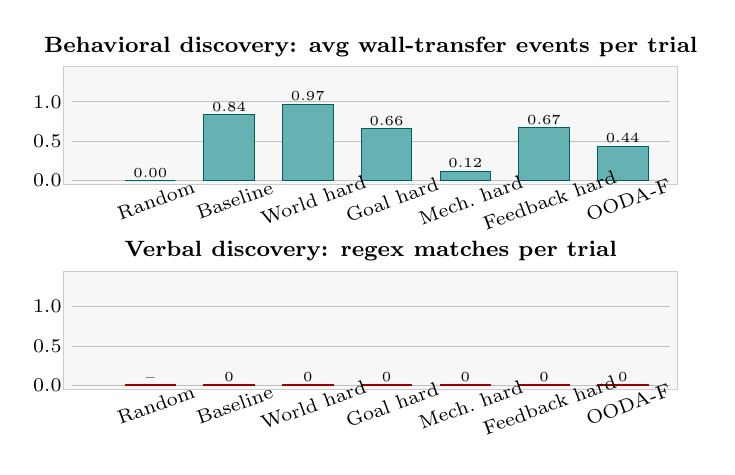
\begin{tikzpicture}[
    bar/.style       ={rectangle, fill=teal!60, draw=teal!75!black, line width=0.3pt},
    barv/.style      ={rectangle, fill=red!50,  draw=red!60!black,  line width=0.3pt},
    bg/.style        ={fill=black!3, draw=black!20, line width=0.3pt},
    ylab/.style      ={font=\scriptsize, anchor=east, inner sep=2pt},
    xlab/.style      ={font=\scriptsize, anchor=north, rotate=20},
    title/.style     ={font=\footnotesize\bfseries, align=center},
    valnum/.style    ={font=\tiny, anchor=south, inner sep=1pt}
  ]
    % --- Common parameters ---
    % data: (config, avg_wt, verbal_rate)
    % Random      n=50  avg_wt=0.00  verbal=0/50
    % Baseline    n=32  avg_wt=0.84  verbal=0/32
    % World hard  n=30  avg_wt=0.97  verbal=0/30
    % Goal hard   n=50  avg_wt=0.66  verbal=0/50
    % Mech hard   n=42  avg_wt=0.12  verbal=0/42
    % Feedback    n=30  avg_wt=0.67  verbal=0/30
    % OODA-F      n=16  avg_wt=0.44  verbal=0/16

    % Vertical scale: 1.0 unit on y = 1.0 wall-transfer/trial
    \def\h{1.0} % height per unit
    \def\bw{0.32} % bar half-width
    % bar centers along x for the 7 conditions
    \def\xrand{0.5}\def\xbase{1.5}\def\xworld{2.5}\def\xgoal{3.5}%
    \def\xmech{4.5}\def\xfeed{5.5}\def\xooda{6.5}

    % background panel
    \draw[bg] (-0.6, -0.05) rectangle (7.2, 1.45);
    \node[title] at (3.3, 1.7) {Behavioral discovery: avg wall-transfer events per trial};

    % y-axis ticks
    \foreach \y/\lab in {0/0.0, 0.5/0.5, 1.0/1.0} {
      \draw[black!25, line width=0.3pt] (-0.5, \y*\h) -- (7.1, \y*\h);
      \node[ylab] at (-0.55, \y*\h) {\lab};
    }

    % bars (behavioral)
    \fill[bar] (\xrand-\bw, 0)  rectangle (\xrand+\bw, 0.00*\h);
    \fill[bar] (\xbase-\bw, 0)  rectangle (\xbase+\bw, 0.84*\h);
    \fill[bar] (\xworld-\bw, 0) rectangle (\xworld+\bw, 0.97*\h);
    \fill[bar] (\xgoal-\bw, 0)  rectangle (\xgoal+\bw, 0.66*\h);
    \fill[bar] (\xmech-\bw, 0)  rectangle (\xmech+\bw, 0.12*\h);
    \fill[bar] (\xfeed-\bw, 0)  rectangle (\xfeed+\bw, 0.67*\h);
    \fill[bar] (\xooda-\bw, 0)  rectangle (\xooda+\bw, 0.44*\h);

    % numeric labels above bars
    \node[valnum] at (\xrand, 0.00*\h) {0.00};
    \node[valnum] at (\xbase, 0.84*\h) {0.84};
    \node[valnum] at (\xworld, 0.97*\h) {0.97};
    \node[valnum] at (\xgoal, 0.66*\h) {0.66};
    \node[valnum] at (\xmech, 0.12*\h) {0.12};
    \node[valnum] at (\xfeed, 0.67*\h) {0.67};
    \node[valnum] at (\xooda, 0.44*\h) {0.44};

    % x-axis labels
    \node[xlab] at (\xrand, -0.05) {Random};
    \node[xlab] at (\xbase, -0.05) {Baseline};
    \node[xlab] at (\xworld, -0.05) {World hard};
    \node[xlab] at (\xgoal, -0.05) {Goal hard};
    \node[xlab] at (\xmech, -0.05) {Mech.\ hard};
    \node[xlab] at (\xfeed, -0.05) {Feedback hard};
    \node[xlab] at (\xooda, -0.05) {OODA-F};

    % --- Verbal panel (below) ---
    \begin{scope}[shift={(0, -2.6)}]
      \draw[bg] (-0.6, -0.05) rectangle (7.2, 1.45);
      \node[title] at (3.3, 1.7) {Verbal discovery: regex matches per trial};

      \foreach \y/\lab in {0/0.0, 0.5/0.5, 1.0/1.0} {
        \draw[black!25, line width=0.3pt] (-0.5, \y*\h) -- (7.1, \y*\h);
        \node[ylab] at (-0.55, \y*\h) {\lab};
      }
      % Every condition: verbal rate = 0/n. Bars are at zero — show as flat baseline.
      \foreach \xc in {\xrand,\xbase,\xworld,\xgoal,\xmech,\xfeed,\xooda} {
        \fill[barv] (\xc-\bw, 0) rectangle (\xc+\bw, 0.012*\h);
      }
      \node[valnum] at (\xrand, 0.012*\h) {--};
      \node[valnum] at (\xbase, 0.012*\h) {0};
      \node[valnum] at (\xworld, 0.012*\h) {0};
      \node[valnum] at (\xgoal, 0.012*\h) {0};
      \node[valnum] at (\xmech, 0.012*\h) {0};
      \node[valnum] at (\xfeed, 0.012*\h) {0};
      \node[valnum] at (\xooda, 0.012*\h) {0};

      \node[xlab] at (\xrand, -0.05) {Random};
      \node[xlab] at (\xbase, -0.05) {Baseline};
      \node[xlab] at (\xworld, -0.05) {World hard};
      \node[xlab] at (\xgoal, -0.05) {Goal hard};
      \node[xlab] at (\xmech, -0.05) {Mech.\ hard};
      \node[xlab] at (\xfeed, -0.05) {Feedback hard};
      \node[xlab] at (\xooda, -0.05) {OODA-F};
    \end{scope}
  \end{tikzpicture}
  \caption{Verbal/behavioral decoupling on \texttt{ka59simple}, aggregated across all model and reasoning settings (counts per Table~\ref{tab:mechanic-triggering}). \emph{Top:} average wall-transfer events per trial varies substantially across conditions, peaking under \texttt{world\_hard} (where models probe most aggressively under degraded observation) and collapsing under \texttt{mechanics\_hard} (action-protocol confound, Appendix~\ref{app:severity}). \emph{Bottom:} the verbal-discovery regex matches \emph{never} fired in any \texttt{ka59simple} cell, including in OODA conditions where the \texttt{orient} field was emitted on every turn. The two metrics are decoupled: behavior carries the mechanic, language does not.}
  \label{fig:decoupling}
\end{figure}

\begin{table}[t]
  \small
  \setlength{\tabcolsep}{4pt}
  \caption{Behavioral and verbal mechanic-triggering on \texttt{ka59simple}, aggregated across model and reasoning settings. ``avg wt'' is wall-transfer events per trial. ``verbal'' is the count of trials in which the discovery regex (Appendix~\ref{app:regex}) fired. The random-agent floor (Section~\ref{sec:random}) produced $0$ wall-transfers across $50$ trials and is included for reference.}
  \label{tab:mechanic-triggering}
  \centering
  \begin{tabular}{lrrrrr}
    \toprule
    Config & $n$ & wins & total wt & avg wt & verbal \\
    \midrule
    Random (uniform)         & 50 &  0 &  0 & 0.00 & --  \\
    Baseline                 & 32 & 20 & 27 & 0.84 &  0  \\
    World hard               & 30 &  0 & 29 & 0.97 &  0  \\
    Goal hard                & 50 & 20 & 33 & 0.66 &  0  \\
    Mechanics hard           & 42 &  0 &  5 & 0.12 &  0  \\
    Feedback hard            & 30 & 16 & 20 & 0.67 &  0  \\
    Mech + OODA              & 10 &  0 &  0 & 0.00 &  0  \\
    Mech + OODA-F            & 16 &  0 &  7 & 0.44 &  0  \\
    \bottomrule
  \end{tabular}
\end{table}

We interpret this as evidence that, on \texttt{ka59simple}, behavioral exploitation of the latent mechanic and verbal articulation of it are decoupled: agents that win do so without verbal discovery, and agents that verbalize discovery often misattribute the mechanic. Self-report-based metrics therefore underestimate behavioral exploitation in this dataset and overestimate the degree of articulated understanding implied by the language.

\subsection{Reasoning effort and OODA-F (exploratory)}
\label{sec:reasoning}
We treat reasoning effort and procedural scaffolding as exploratory secondary factors. On \texttt{ka59simple}, neither uniformly helps nor hurts. Within GPT-5.2, medium reasoning improves baseline ($4/5 \to 5/5$) but reduces \texttt{goal\_hard} ($6/10 \to 2/10$); Grok-4.1-fast shows the inverse on \texttt{goal\_hard} ($2/10 \to 7/10$). At $n=10$ the within-family Wilson 95\% CIs still overlap, but the cross-family direction reversal is visible at the point-estimate level---a $40$pp drop with reasoning effort for GPT-5.2 versus a $50$pp rise for Grok on the same axis.

\paragraph{OODA-F.} The OODA-F scaffold (Appendix~\ref{app:prompts}) is a procedural prompt intervention adapted from Boyd's military \emph{Observe / Orient / Decide / Act} decision loop: it requires the agent to emit a structured \texttt{observe} / \texttt{orient} / \texttt{decide} / \texttt{action} JSON object every turn, plus a \emph{forced-reframe} directive that activates after several turns of stalled behavior and instructs the agent to discard its current hypothesis and switch action types. The intent is to elicit explicit hypothesis revision under a partial-observability task; we use it precisely because verbal hypothesis revision is what the verbal-discovery indicator was supposed to detect. Across $16$ OODA-F trials on \texttt{mechanics\_hard}, the scaffold elicited forced reframes on $24\%$ of turns on average and produced $7$ wall-transfer events, but yielded $0$ wins. This null result is consistent with the verbal/behavioral decoupling of Section~\ref{sec:verbal-behavioral}: triggering more articulate hypothesis revision does not, on its own, produce the multi-step plan needed to exploit the mechanic.

\section{Limitations}
\label{sec:limits}
\paragraph{Sample size.}
Most non-\texttt{goal\_hard} cells are $n=5$; \texttt{goal\_hard} cells were extended to $n=10$ in a follow-up batch reported here. We report Wilson 95\% intervals throughout; many comparisons we discuss have overlapping intervals and should be treated as exploratory rather than confirmatory.

\paragraph{Single-environment headline.}
The attributed comparison runs on \texttt{ka59simple}, a constructed single-goal variant we built to escape the canonical KA59 floor effect. We are explicit that \texttt{ka59simple} is a methodological tool, not a benchmark replacement; cross-environment generality of the verbal/behavioral decoupling is not yet established. BP35 and LS20 supporting evidence is GPT-5.2-only.

\paragraph{Knockout severity is binary.}
Each axis is operationalized as a complete present/absent ablation, not a graded reduction. Some findings (\texttt{world\_hard} collapses performance) are then partly entailed by the design rather than fully empirical. Findings on the mechanics axis are additionally confounded with action-protocol absence in \texttt{MECHANICS\_HARD}; we disclose the prompt deltas in Appendix~\ref{app:severity}.

\paragraph{Verbal-discovery regex is heuristic.}
Our regex is a falsifiable but unvalidated estimator. Its zero-match rate on \texttt{ka59simple} is informative as a direction of disagreement with behavior, not as a calibrated belief estimator. We have not benchmarked precision/recall against human annotation; we treat the metric as conservative for ``unambiguous push-through articulation,'' not for ``has the agent inferred anything.''

\paragraph{Pre-fix reasoning-effort cells.}
A subset of GPT-5.2 cells were collected before a per-handler bug in the OpenRouter \texttt{reasoning\_effort} forwarding path was fixed. Those cells map to provider-default reasoning rather than to a controlled level. They are excluded from the main body and reported in Appendix~\ref{app:cells}. The fix and a probe verifying the post-fix path are described there.

\paragraph{Cross-family scope.}
Only two model families are represented (GPT-5.2 and Grok-4.1-fast), both via OpenRouter. Open-weight baselines and Anthropic models with matched reasoning controls are absent. Cross-family interpretation is descriptive rather than causal.

\paragraph{LS20 \texttt{world\_hard} outlier.}
GPT-5.2 with no reasoning achieves $3/5$ on LS20 \texttt{world\_hard} despite the otherwise consistent collapse. Trace inspection of those runs is planned to determine whether this reflects environment-specific world-model robustness or a heuristic shortcut in LS20's geometry.

\paragraph{Random-agent floors for BP35 and LS20.}
Section~\ref{sec:random} reports random-agent floors only for KA59 and \texttt{ka59simple}, the two environments whose source files are present in our shared repository. BP35 and LS20 are owned by other authors in separate lane branches; running our random-agent harness against those environments requires their lane-owners' environment files and is listed as straightforward follow-up work. A reviewer wishing to cross-check should expect comparable floor estimates given the action-space similarities, but we do not assert this without measurement.

\paragraph{\texttt{ka59simple} geometry: incidental vs.\ intentional mechanic use.}
The two selectables in \texttt{ka59simple} are placed on the same horizontal row, with the wall and goal both to the right of the player's spawn. As a result, an agent that simply moves right toward the visible goal will frequently push the second selectable into the wall and trigger a wall-transfer event without explicitly planning for it. Inspecting winning trials shows that wall-transfer events are sometimes \emph{incidental} (the agent moves right, the engine produces a teleport, the agent's stated reasoning does not anticipate it), although the subsequent \texttt{CLICK} on the post-wall sprite---which every win requires---is itself a deliberate action that the agent must select after noticing the transferred piece. Our \texttt{wall\_transfers} metric therefore overstates intentional mechanic use, and the verbal/behavioral decoupling result of Section~\ref{sec:verbal-behavioral} should be read as: agents win by executing a sequence that includes both an incidental push and a deliberate click-switch, while never verbalizing either step. A revised geometry that places the player and second selectable on different rows---so an agent must plan a vertical detour to engage the wall-transfer mechanic---would isolate intentional from incidental use and is a natural next variant.

\section{Conclusion}
We present a four-axis knockout framework that grounds each axis in a specific component of an underlying POMDP, and we report a KA59-centered empirical study with explicit Wilson confidence intervals, a uniform-random floor reference, and a behavioral-vs.-verbal discovery analysis. Two outcome-level findings are robust across model families and reasoning settings on \texttt{ka59simple}: world- and mechanics-axis ablations collapse performance to $0\%$ wins, with random-agent floor at $0\%$ as a calibrating reference. The most novel finding is at the trace level: across all $210$ \texttt{ka59simple} trials, behavioral exploitation of the wall-transfer mechanic and verbal articulation of it decouple completely---agents win without verbalizing discovery, agents that verbalize misattribute, and a procedural OODA-F scaffold does not close the gap. BP35 and LS20 supporting evidence is consistent with the world-axis collapse pattern for GPT-5.2, but cross-family and reasoning-effort claims do not yet extend to those environments. We interpret these results as evidence that hidden-mechanic discovery is a distinct capability axis on which self-report-based discovery metrics systematically underestimate behavioral exploitation, and that benchmarks for interactive agents under partial observability should pair outcomes with mechanism-specific behavioral signals rather than rely on stated hypotheses alone.

\bibliographystyle{plainnat}
\bibliography{references}

\appendix

\section{Environment specifications}
\label{app:envs}
\paragraph{Canonical KA59.}
The canonical version is loaded from the obfuscated game source at \texttt{environment\_files/ka59/38d34dbb/ka59.py} via the \texttt{arc\_agi} Arcade harness. It exposes seven levels; we restrict to level~1 throughout. Level~1 contains two selectables at cell positions $(9, 21)$ and $(18, 21)$, two goal tiles at $(2, 23)$ and $(35, 17)$, a wall block centered at $(24, 12)$, and a letterbox sentinel object that does not affect agent decisions. The action space is $\{\texttt{MOVE\_UP}, \texttt{MOVE\_DOWN}, \texttt{MOVE\_LEFT}, \texttt{MOVE\_RIGHT}, \texttt{CLICK}\}$. \texttt{MOVE\_*} attempts a $3$-pixel shift of the currently selected piece in the corresponding direction; \texttt{CLICK} expects a \texttt{target\_position} field and switches selection to the selectable at that grid coordinate, if one exists. The win condition is \emph{simultaneous} occupancy of every goal tile by a selectable.

\paragraph{Hidden wall-transfer asymmetry.}
The engine's player-move handler checks for wall tags and silently reverts blocked moves. The recursive push handler used to propagate motion through pushed objects checks only for solid letterboxes and selectable collisions; it does \emph{not} check the wall tag. As a consequence, when the player's \texttt{MOVE\_*} would push a second selectable into a wall, the pushed sprite is teleported across the wall (a $+15$-pixel jump in the engine's $3$-pixel grid). None of the agent-facing prompts describe this asymmetry.

\paragraph{\texttt{ka59simple}.}
\texttt{ka59simple} (located at \texttt{environment\_files/ka59simple/20260430/}) is a single-level fork of canonical KA59 level~1, constructed by removing the left-side goal tile while preserving both selectables, the wall block, the letterbox, and the engine's wall-transfer asymmetry. The optimal solve is six actions: three \texttt{MOVE\_RIGHT} (pushing the second selectable through the wall), one \texttt{CLICK} on the transferred sprite at $(33, 21)$, then \texttt{MOVE\_RIGHT} and \texttt{MOVE\_UP} to enter the goal at $(35, 17)$. The right selectable cannot reach the goal without the wall-transfer mechanic.

\paragraph{BP35 and LS20.}
Both environments share the four-axis condition definitions described in Section~\ref{sec:method} but expose different latent mechanics and goal structures. We do not redescribe their internals here; their owners' lane code is available alongside our harness. For the present paper, BP35 and LS20 results are used only as supporting cross-environment evidence under GPT-5.2 (no, medium) and GPT-4.1 (no).

\section{Full prompts}
\label{app:prompts}
The system prompt assembled for each condition concatenates the goal and mechanics components defined in \texttt{ka59\_game/prompts.py}. Per-turn user prompts contain the recent action history, a status block (selected piece, level, steps remaining), and a per-condition observation block.

\paragraph{\texttt{GOAL\_EASY}.}
\begin{verbatim}
Your goal is to complete the KA59 puzzle game by progressing through all of its
levels. Each level presents a grid with obstacles, one or more selectable
pieces, and one or more goal tiles marked `+` in the semantic grid. You win a
level by placing each selectable piece onto a goal tile. If a level has
multiple goal tiles, EVERY goal must be occupied by a selectable piece
simultaneously for the engine to report WIN. Once the run reports WIN, the
whole game is won. Use actions efficiently; the step budget per level is
finite.
\end{verbatim}

\paragraph{\texttt{GOAL\_HARD}.}
The empty string. The agent receives no description of what counts as winning.

\paragraph{\texttt{MECHANICS\_EASY}.}
\begin{verbatim}
Game mechanics:
- Positions are `[x, y]` pixel coordinates. x increases rightward, y increases
  downward.
- The grid uses 3 pixels per cell. Movement actions attempt to shift the
  currently selected piece in the chosen direction; interactions with certain
  objects or boundaries may produce unexpected results.
- Some objects are pushable: if a pushable object is immediately adjacent in
  the movement direction, a push may occur (the pushable shifts along with the
  selected piece).
- Some objects are walls. Walls may block movement in various ways. Not all
  wall-like boundaries behave identically -- you must interact with them to
  discover their behavior.
- A level can contain more than one selectable piece. Use `CLICK` with a
  `target_position` to switch control to another selectable piece at that
  position. `target_position` must be given in the SAME coordinates as
  `player.position` and every entry in `objects` -- i.e. the pixel/grid
  coordinates shown in the state dict, NOT cell indices from the
  semantic_grid.

Observation each turn:
- `player.position` and `player.id` identify the currently selected piece.
- `movement.{direction}_blocked` is a heuristic hint (True if there is any
  adjacent object in that direction). It does NOT guarantee an action will
  fail -- try it to learn.
- `objects.{walls,blocks,selectables,goals}` lists every on-screen object's
  position and size.
- `semantic_grid` is a compact ASCII picture of the current cell-grid:
  P=selected, S=other selectable, B=block, #=wall, +=goal, .=empty.
- `level.current` / `level.total` show your progress.
  `resources.steps_remaining` is the per-level budget.

Response protocol:
Each turn, respond with a single JSON object only:
{"reasoning": "<1-2 sentences>", "action": "MOVE_RIGHT"}

For CLICK, include target_position in the SAME coordinates as
`player.position`:
{"reasoning": "Switch to the other selectable at [18, 21].",
 "action": "CLICK", "target_position": [18, 21]}

Valid actions:
- `MOVE_LEFT`
- `MOVE_RIGHT`
- `MOVE_UP`
- `MOVE_DOWN`
- `CLICK` with `"target_position": [x, y]` in grid/pixel coordinates (same
  system as `player.position` and `objects.*[*].position`)
\end{verbatim}

\paragraph{\texttt{MECHANICS\_HARD}.}
\begin{verbatim}
Respond each turn with a JSON object only:
{"action": "<chosen action>", "target_position": [x, y] if CLICK}
\end{verbatim}

\paragraph{\texttt{MECHANICS\_OODA} (procedural-mechanics variant).}
\begin{verbatim}
Each turn, respond with a JSON object only using this exact structure:
{"observe": "<what changed since last turn>",
 "orient":  "<your current hypothesis about how this world works>",
 "decide":  "<what you will do and why>",
 "action":  "<ACTION_NAME>",
 "target_position": [x, y] if CLICK}

For your first turn, set observe to your initial reading of the state.
Update your orient hypothesis every turn based on outcomes -- if something
unexpected happened, revise it.
Valid actions: MOVE_LEFT, MOVE_RIGHT, MOVE_UP, MOVE_DOWN, CLICK
\end{verbatim}

\paragraph{\texttt{MECHANICS\_OODA\_F} (forced-reframe variant).}
\begin{verbatim}
Each turn, respond with a JSON object only using this exact structure:
{"observe": "<what changed since last turn>",
 "orient":  "<your current hypothesis about how this world works>",
 "decide":  "<what you will do and why>",
 "action":  "<ACTION_NAME>",
 "target_position": [x, y] if CLICK}

For your first turn, set observe to your initial reading of the state.
Update your orient hypothesis every turn based on outcomes -- if something
unexpected happened, revise it.
Valid actions: MOVE_LEFT, MOVE_RIGHT, MOVE_UP, MOVE_DOWN, CLICK

IMPORTANT: When you see a [FORCED REFRAME] notice in the observation, your
recent strategy has not made progress. You MUST: (1) discard your current
hypothesis entirely, (2) state a new hypothesis based solely on what you have
actually observed, (3) choose a completely different action type than what
you have been using.
\end{verbatim}

\paragraph{\texttt{FEEDBACK\_HARD}.}
The literal string \texttt{"Ok."}. Replaces the per-turn outcome description (which under \texttt{FEEDBACK\_EASY} compares pre- and post-state to summarize what changed).

\paragraph{Per-turn user prompt structure (\texttt{WORLD\_EASY}).}
\begin{verbatim}
RECENT ACTIONS (last 10 turns):
Turn k: <ACTION>
  Result: <feedback>
...

STATUS:
Selected: <id> @ <position>
Level: <current>/<total>
Steps remaining this level: <int>

CURRENT STATE (turn t/<max>):
<JSON state dict, see WORLD_EASY below>

SEMANTIC LEGEND: ...
SEMANTIC GRID (indexed): ...

Respond with a single JSON object only: {"reasoning": ..., "action": ...}
\end{verbatim}

\paragraph{Observation deltas under each axis.}
\texttt{WORLD\_HARD} replaces the full state dict with a minimal projection containing only \texttt{player}, \texttt{movement} blocked-flags, \texttt{level}, \texttt{resources}, \texttt{game\_state}, and per-category \emph{counts} of objects (no positions, no goal locations). \texttt{FEEDBACK\_HARD} replaces the per-turn ``Result: \dots'' description with \texttt{"Ok."}. \texttt{GOAL\_HARD} and \texttt{MECHANICS\_HARD} affect the system prompt only.

\section{Knockout severity disclosure}
\label{app:severity}
We deliberately operationalize each axis as a complete binary ablation. Below we list the exact semantics and the design confounds we are aware of.

\paragraph{World.}
\texttt{EASY}: full structured state including the semantic grid; \texttt{HARD}: only the selected piece's position, blocked flags, level/budget counters, and per-category counts. \emph{Confound:} \texttt{HARD} hides goal locations entirely, so \texttt{world\_hard} collapse on goal-occupancy tasks is partly entailed by the design. We treat the magnitude of the collapse, not its sign, as the empirical question.

\paragraph{Goal.}
\texttt{EASY}: a description of the win condition; \texttt{HARD}: the empty string. \emph{Confound:} the agent has no out-of-band hint that there is a goal at all---some failures may stem from the agent treating the run as an unprompted exploration task. The remaining win rate under \texttt{goal\_hard} is therefore particularly informative.

\paragraph{Mechanics.}
\texttt{EASY}: a description of the coordinate system, push semantics, wall hint, multi-selectable / \texttt{CLICK} semantics, observation schema, and response protocol; \texttt{HARD}: a one-line response-format instruction only. \emph{Confound:} \texttt{HARD} also removes the description of the \texttt{CLICK} \texttt{target\_position} protocol. Agents under \texttt{mechanics\_hard} who emit \texttt{CLICK} without valid \texttt{target\_position} are scored as invalid actions; this is partly an action-grammar effect rather than a pure mechanics-discovery effect, and we report it accordingly.

\paragraph{Feedback.}
\texttt{EASY}: a per-turn narrative summary of what changed (positions, selection, blocked outcomes); \texttt{HARD}: the literal string \texttt{"Ok."}. \emph{Confound:} the underlying observation still updates, so \texttt{feedback\_hard} measures the loss of \emph{narrative} feedback specifically, not the loss of all signal.

\section{Discovery regex specification}
\label{app:regex}
The verbal-discovery regex (\texttt{check\_discovery} in \texttt{ka59\_game/prompts.py}) is composed of positive patterns and explicit veto patterns. Both lists are case-insensitive.

\paragraph{Positive patterns (any match counts as candidate discovery).}
\begin{verbatim}
through the wall
push(?:ed|ing)? through
different for push
wall[^.]{0,60}\b(?:is|are|may\s+be|could\s+be|might\s+be|appears?\s+to\s+be)
       \s+passable
wall[^.]{0,60}permeable
wall[^.]{0,30}not\s+(?:solid|blocking|blocked|impassable)
see\s+if\s+the\s+wall\s+is\s+passable
(?:wall|push).{0,40}asymmetr
asymmetr.{0,40}(?:wall|push)
(?:move|push).{0,60}block.{0,40}(?:cross|pass).{0,20}wall
pushed block pass
\end{verbatim}

\paragraph{Veto patterns (any match disqualifies the candidate).}
\begin{verbatim}
click.{0,80}(?:teleport|transfer|cross|jump).{0,60}wall
(?:teleport|transfer|jump).{0,60}click
select.{0,60}transfer
transfer.{0,60}select
(?:no\s+(?:path|way)|cannot|can.t|unable)\s*.{0,30}through\s+the\s+walls?
\end{verbatim}

\paragraph{Validation note.}
We have not benchmarked precision/recall against human annotation. The regex is intentionally conservative for ``unambiguous push-through articulation'' and intentionally vetoes \texttt{CLICK}-based misattribution language. Its zero-match rate on \texttt{ka59simple} ($n=210$ trials, $1{,}544$ \texttt{orient} entries) is therefore informative as a direction-of-disagreement statistic with behavior, not as a calibrated belief estimator.

\section{Per-cell numbers and the pre-fix \texttt{5.2 dflt} cells}
\label{app:cells}
Table~\ref{tab:dflt-cells} reproduces the GPT-5.2 omitted-default ($5.2~\text{dflt}$) cells excluded from the main body. These cells were collected via OpenRouter before a per-handler bug in the \texttt{reasoning\_effort} forwarding path was identified and fixed; they map to provider-default reasoning ($\sim$minimal/low for GPT-5.2) rather than to a controlled level. We retain them here for completeness and so that any reader who wishes to cross-check our pre-fix data against external sources can do so.

\begin{table}[h]
  \small
  \setlength{\tabcolsep}{4pt}
  \caption{Pre-fix GPT-5.2 omitted-default \texttt{ka59simple} cells, with Wilson 95\% intervals.}
  \label{tab:dflt-cells}
  \centering
  \begin{tabular}{lc}
    \toprule
    Config & 5.2 dflt \\
    \midrule
    Baseline       & 6/10 [31,83] \\
    World hard     & 0/10 [0,28] \\
    Goal hard      & 3/10 [11,60] \\
    Mechanics hard & 0/10 [0,28] \\
    Mech + OODA-F  & 0/6 [0,39] \\
    \bottomrule
  \end{tabular}
\end{table}

\paragraph{Bug summary and verification.}
The OpenRouter handler in \texttt{ka59\_game/llm\_client.py} historically did not forward the \texttt{reasoning\_effort} kwarg into the per-request body, so any \texttt{--reasoning-effort none} or \texttt{medium} flag was silently dropped on that path. The fix uses OpenRouter's unified \texttt{extra\_body=\{"reasoning": \{"effort": \dots\}\}} form, which is supported across OpenRouter's OpenAI, xAI, and Anthropic provider routes. We verified the fix by running \texttt{scripts/probe\_reasoning\_effort.py}, which inspects \texttt{usage.completion\_tokens\_details.reasoning\_tokens} for the same prompt across effort levels. On a controlled $303$-token KA59-style prompt, the post-fix probe returned $0$ reasoning tokens for \texttt{effort=none} and $1{,}240$ reasoning tokens for \texttt{effort=medium}, confirming end-to-end that the flag now reaches the model. The pre-fix \texttt{5.2 dflt} cells in Table~\ref{tab:dflt-cells} are internally consistent (every trial at the same effective default-reasoning level for that model) but should not be compared to similarly-labelled cells from other models, since per-model defaults differ ($\approx$ \texttt{minimal} for GPT-5.2 via this provider; near-default \texttt{high} for Grok-4.1-fast). All cells reported in the main body of this paper are post-fix.

\section{Trace case studies}
\label{app:traces}
We reproduce three \texttt{orient\_history} excerpts to illustrate the verbal/behavioral decoupling reported in Section~\ref{sec:verbal-behavioral}. All three are abbreviated for length; the source JSONs are available alongside the harness.

\paragraph{Case 1: behavioral discovery without verbal discovery (win).}
\texttt{ka59simple} baseline run, GPT-5.2 explicit no-reasoning, $16$ turns, $2$ wall-transfer events, $1/1$ goals occupied, regex did not fire (and indeed the run was not in OODA mode, so no \texttt{orient} field was emitted). The agent solved the puzzle in roughly the optimal sequence---three \texttt{MOVE\_RIGHT} pushes that triggered the wall-transfer mechanic, followed by a \texttt{CLICK} switching to the transferred sprite, then \texttt{MOVE\_RIGHT} and \texttt{MOVE\_UP} to enter the goal---without producing the language the regex looks for. The post-run \texttt{UNDERSTANDING} prompt elicited the following self-report on mechanics:
\begin{quote}\itshape
``Movement actions (up/down/left/right) move the currently selected piece in $3$-pixel grid steps $\dots$ Moves can be blocked by walls or other objects, though the movement-blocked flags are only hints and don't guarantee failure. Some adjacent objects (blocks) can be pushed if immediately next to the selected piece in the movement direction $\dots$''
\end{quote}
The agent describes movement and pushing in language that paraphrases \texttt{MECHANICS\_EASY} but does not articulate the wall-transfer asymmetry it just exploited twice to win the level. Across all $56$ \texttt{ka59simple} wins in our dataset, no \texttt{UNDERSTANDING} response we hand-checked attributes the win to push-through-wall behavior; agents instead describe walls as generally blocking and pushing as ordinary one-cell shifts.

\paragraph{Case 2: verbal misattribution under OODA (loss).}
Canonical KA59 \texttt{mech\_ooda} trial, GPT-5.2, $64$-turn budget, $0$ wall-transfer events recorded, regex \emph{fired} on turn $9$. The \texttt{orient} field at the time of the match read, in part, ``CLICK on an empty/open position teleports the selected piece $\dots$ the world has multiple selectable pieces. One is always selected (player). CLICK $[x,y]$: if $[x,y]$ contains an unselected selectable, transfers selection to it.'' The agent's hypothesis attaches the transfer language to \texttt{CLICK} (selection switching), not to the wall-transfer mechanic actually responsible for the empirically larger jumps. The veto patterns are designed to suppress this kind of language but in this trace the wording slipped past.

\paragraph{Case 3: OODA-F null (loss).}
\texttt{ka59simple} \texttt{mechanics\_ooda\_f} trial, $32$-turn budget, $0$ wall-transfer events, $4$ forced reframes triggered. After each forced reframe, the agent emitted a new \texttt{orient} hypothesis but reverted to repeating the same action types within a small number of turns. The regex did not fire. This trace, together with $15$ similar OODA-F trials, accounts for the $0/16$ wins reported in Section~\ref{sec:reasoning}: the procedural scaffold elicits articulated hypothesis revision but does not, on its own, produce the multi-step plan needed to exploit the latent mechanic.

\section{Reproducibility}
\label{app:repro}
The harness, environment files for KA59 and \texttt{ka59simple}, and the analysis scripts used to produce the tables in this paper are all in the project repository. Below we list the entry-point commands. All runs use OpenRouter for LLM calls; the random baseline does not require any API key.

\paragraph{Random-agent floor (no LLM).}
\begin{verbatim}
# ka59simple, 32-turn budget, n=50:
python3 -m scripts.run_random_baseline --env ka59simple \
    --trials 50 --max-turns 32 --seed 0

# canonical KA59, 50-turn budget, n=30:
python3 -m scripts.run_random_baseline --env ka59 \
    --trials 30 --max-turns 50 --seed 1
\end{verbatim}

\paragraph{Single-cell ablation sweep (LLM).}
\begin{verbatim}
# explicit no-reasoning GPT-5.2 baseline + four single-axis knockouts:
python3 -m scripts.run_real_ablation \
    --env ka59simple --provider openrouter --model openai/gpt-5.2 \
    --reasoning-effort none --trials 5 --max-turns 32 \
    --configs baseline world_hard goal_hard mechanics_hard feedback_hard

# Grok-4.1-fast medium-reasoning, same configs:
python3 -m scripts.run_real_ablation \
    --env ka59simple --provider openrouter --model x-ai/grok-4.1-fast \
    --reasoning-effort medium --trials 5 --max-turns 32 \
    --configs baseline world_hard goal_hard mechanics_hard feedback_hard
\end{verbatim}

\paragraph{Wilson 95\% confidence intervals.}
\begin{verbatim}
python3 scripts/wilson_cis.py
\end{verbatim}

\paragraph{Per-trial JSONs and aggregates.}
Each trial writes a per-trial JSON to \texttt{results/<env>\_game/run\_*.json} containing the full event history, \texttt{orient\_history}, action timeline, and end-of-run \texttt{understanding} response. Aggregated cell-level summaries are in \texttt{results/<env>\_real\_ablation/ablation\_*.json}. Random-agent runs write to the same \texttt{results/<env>\_real\_ablation/} directory under \texttt{random\_baseline\_*.json}.

\paragraph{OpenRouter \texttt{reasoning\_effort} probe.}
The probe in \texttt{scripts/probe\_reasoning\_effort.py} verifies that the OpenRouter handler in \texttt{ka59\_game/llm\_client.py} forwards \texttt{reasoning\_effort} correctly by inspecting \texttt{usage.completion\_tokens\_details.reasoning\_tokens} across explicit \texttt{none}, default, and \texttt{medium} settings. We re-ran this probe before each batch reported in the main body.

\newpage
\input{checklist.tex}

\end{document}
